\documentclass[UTF8, a4paper, 11pt]{article}
\usepackage{fontspec}
\usepackage{float}
\usepackage{amsmath}
\usepackage{graphicx}
\usepackage{geometry}
\usepackage{listings}
\usepackage{xcolor}
\usepackage{caption,subcaption}
\geometry{scale=0.8}
\linespread{1.5}
\usepackage{hyperref}
\usepackage{color}
\usepackage{fontspec}
\usepackage{enumitem}
\usepackage[linesnumbered,boxed]{algorithm2e}    
\usepackage{xeCJK}
\usepackage{indentfirst} 
\graphicspath{{Pics/}} 	% 在于.tex同级的目录下创建名为pic的文件夹,存放图片


\setlength{\parindent}{2em}

\lstset{
language={Python},
frame=shadowbox,
breaklines=true,
 numbers=left,
 backgroundcolor=\color[RGB]{245,245,244},
 rulesepcolor=\color{red!20!green!20!blue!20},
 numberstyle={\color[RGB]{0,192,192}\tiny},
 basicstyle=\footnotesize \fontspec{Source Code Pro}
 }
\setenumerate[1]{itemsep=0pt,partopsep=0pt,parsep=\parskip,topsep=0pt}
\setitemize[1]{itemsep=0pt,partopsep=0pt,parsep=\parskip,topsep=0pt}
\setdescription{itemsep=0pt,partopsep=0pt,parsep=\parskip,topsep=0pt}


\title{	
\normalfont \normalsize
\textsc{School of Data and Computer Science, Sun Yat-sen University} \\ [25pt] %textsc small capital letters
\rule{\textwidth}{0.5pt} \\[0.4cm] % Thin top horizontal rule
\huge  Language Model\\ % The assignment title
\rule{\textwidth}{2pt} \\[0.5cm] % Thick bottom horizontal rule
\author{18308045 Zhengyang Gu}
\date{\normalsize\today}
}

\begin{document}
\maketitle
\tableofcontents
\newpage

\section{Abstract}
The language model is implemented through LSTM and the effects of hyperparameters is discussed in the report.

\section{Background}
\subsection{LSTM}
The LSTM was introduced in the last report.
Briefly, the most advantage of it over the simplest RNN is that it can forget like humans do.
However, I do not use the BiLSTM here but LSTM to implement the language model,
because when generating a new word, the words after the new word is unkown and should not be considered.
\subsection{Cross Entropy}
The typical form of cross entropy is given by:
$$H(p,q)=-\sum_x p(x) \log(q(x))$$
where the $x$ an assignment of a feature,
$p$ is the actual probability distribution of the feature and the $q$ is the predicted probability distribution of the feature.
When the two distribution are similar, the cross entropy between them is low.

\section{Implementation}
\subsection{Training}
The idea behind the language model is simple. The feature here is the current word and the domain of it is all of the words that appear in the training set.
The model is fed with the last hidden state and the last word of the sentence and generate a predicted probability distribution of the word
which has the form of vector filled with probabilities and a new hidden state. And we choose the word with the highest probability to be the current predicted word.
The loss here is the cross entropy between the actual probability distribution which has the form of one-hot vector and the predicted probability distribution.
We want to minimize the loss to make the predicted probability distribution be as similar to the actual probability distribution as possible in order to get
a humman-like prediction of the current word based on words in the sentence before the current word.
\begin{lstlisting}
hidden_batch = None
output_batch = model(inputs_batch.to(device), hidden_batch)[0]
loss = cross_entropy_loss(output_batch.reshape(-1, len(ix2word)),
							outputs_batch.to(device).reshape(-1))
loss.backward()
\end{lstlisting}

\subsection{Testing}
I use the average loss of the every sentence in the training set but not the accuracy to observe its convergence.
The reason is that our goal is to get a prediction that is humman-like which means we just need to get a relatively similar probability distribution of
the current word but not a predicted word that is completely same as the word in the training set, and the accuracy can be very slow.
And I test the loss sperately. It is because here I exploit the batch to speed up the training process,
and it's hard to average the loss calculated during this process because of padding.
Though it costs a lot of time to calculate the loss with batch size 1, there's no need to calculate the gradient of the loss and to update weights so it's not as
time-consuming as the training with batch size 1.

Additionaly, I wrote a script which get a word as the input and output a sentence. We can evaluate the model by just evaluate how fluent the sentence is.

\section{Result}
\subsection{Small Training Set}
I first trained the model on a training set with only 3000 sentences. The hyperparameters I set are shown as follows.
\begin{lstlisting}
BATCH_SIZE = 32
EMBEDDING_DIM = 128
HIDDEN_DIM = 128
\end{lstlisting}

And I tested different learning rate. The result is as follows.
\begin{figure}[H]
      \centering
      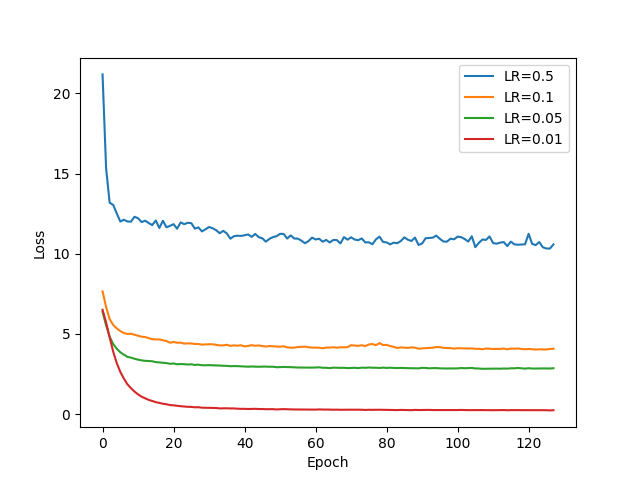
\includegraphics[width = 0.8 \textwidth]{loss3000.png}
\end{figure}
The result shows that the model trained with the learning rate of 0.01 has the best performance.

I inputed some common words to the model trained with the learning rate of 0.01 and with 128 epochs. The result it generated is as follows.
\begin{figure}[H]
      \centering
      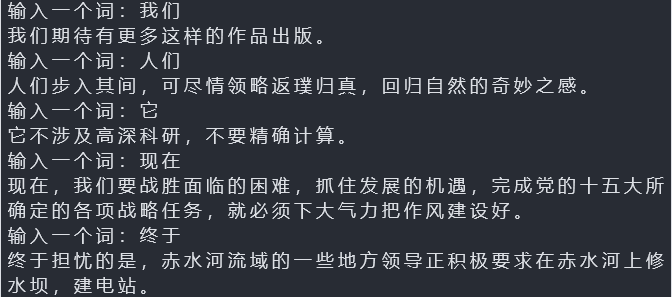
\includegraphics[width = 0.8 \textwidth]{test3000.png}
\end{figure}
These sentences are quite fluent, but some of them are exactly same as sentences in training set. The reason of it may be that the size of training set is too small.

\subsection{Large Training Set}
Then I trained the model on the whole training set which has almost 100000 sentences. The hyperparameters I set are shown as follows.
\begin{lstlisting}
BATCH_SIZE = 16
EMBEDDING_DIM = 128
HIDDEN_DIM = 128
\end{lstlisting}
But the loss of it ascend which is quite abnormal. At first I thought the reason might be that the number of words got larger while the size of the word embedding
and the hidden state do not got larger. Therefore I tried enlarging the size of the word embedding the hidden state. However, the loss ascend even faster.
\begin{figure}[H]
      \centering
      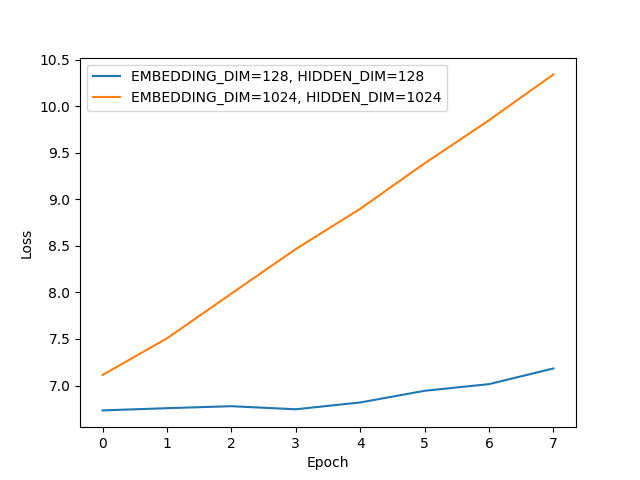
\includegraphics[width = 0.8 \textwidth]{1024.png}
\end{figure}
Then I thought that maybe it was the learning rate that is so small that cause the overshooting problem.
\begin{figure}[H]
      \centering
      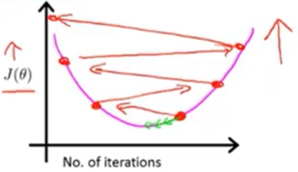
\includegraphics[width = 0.8 \textwidth]{overshoot.png}
\end{figure}
Therefore I tried decrease the learning rate. The loss finally went down.
\begin{figure}[H]
      \centering
      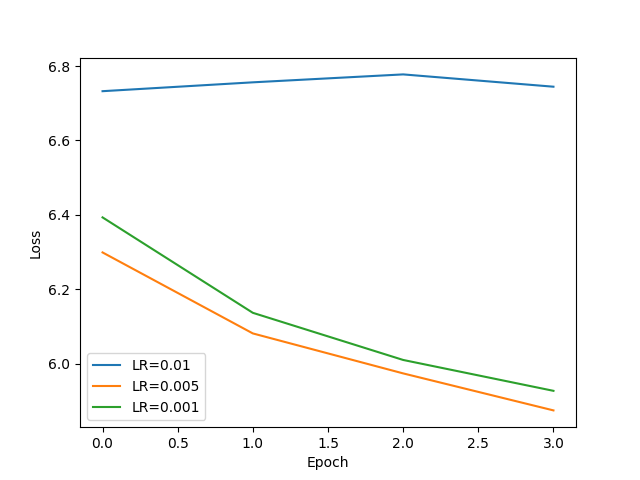
\includegraphics[width = 0.8 \textwidth]{low_lr.png}
\end{figure}
Then I used the learning rate of 0.005 to proceed the training.
\begin{figure}[H]
      \centering
      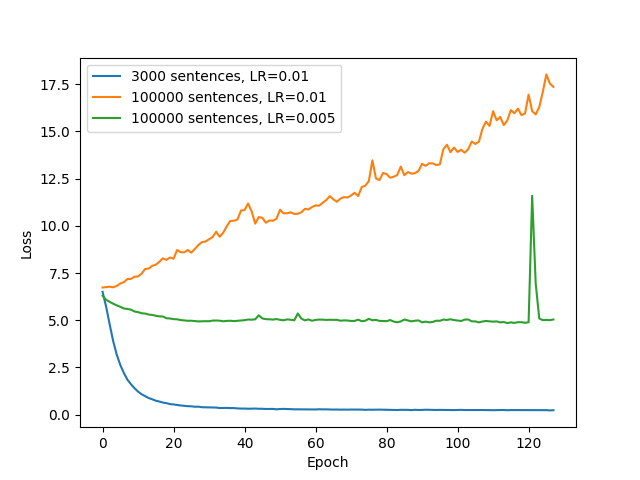
\includegraphics[width = 0.8 \textwidth]{loss100000.png}
\end{figure}
The loss's sudden ascent maybe mean that it just miss a locally optimal solution. Therefore I inputed some words in the model trained with 120 epochs which is a
relatively good solution which is also relatively close to the locally optimal solution.
\begin{figure}[H]
      \centering
      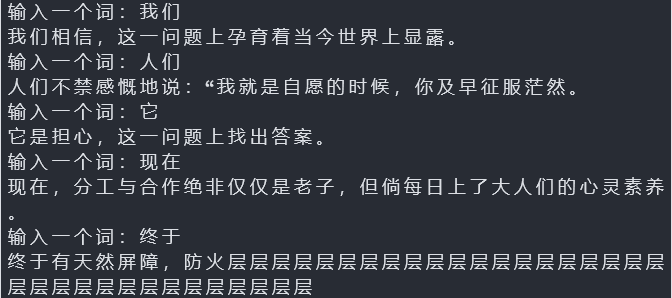
\includegraphics[width = 0.8 \textwidth]{test100000.png}
\end{figure}
These sentences are absolutely not from training set but they are not fluent as the sentences generated by the model trained with 3000 sentences.

\section{Conclusions And Bonuses I May Get}
\begin{enumerate}
      \item I implemented a language model using LSTM.
      \item I use batch and GPU to speed up the training process.
      \item I discussed the effects of hyperparameters.
      \item I compose my report in English, although it may be not fluent.
\end{enumerate}

Future work may include the experiment with more running epochs.
%\clearpage
%\bibliography{E:/Papers/LiuLab}
%\bibliographystyle{apalike}
\end{document} 
%%% Local Variables:
%%% mode: latex
%%% TeX-master: t
%%% End:
